
\label{chap:software-operations_Gardener}


\subsection{Ask for a diffrent seed}

\hrule
\hfill
\vspace{0.5cm}

\label{operation:Ask for a diffrent seed}

The gardener can request a diffrent seed which isn't already in the crops
inventory.
\begin{description}
\item \textbf{Parameters:} SeedName,Amount
\item \textbf{Precondition:} The system is bootedup and the Gardener has to be
logged in and be on the Gardener screen.
\item \textbf{Post-condition:} The request has been send by adding it on the
request seed table.
\item \item \textbf{Output messages:}Reqeust has been send.
\item \textbf{Triggering:}
\begin{enumerate}
\item \textbf{Gardener} complets the diffrent input text fields and presses
the ask for a non existing seed button.
\begin{figure}[H]
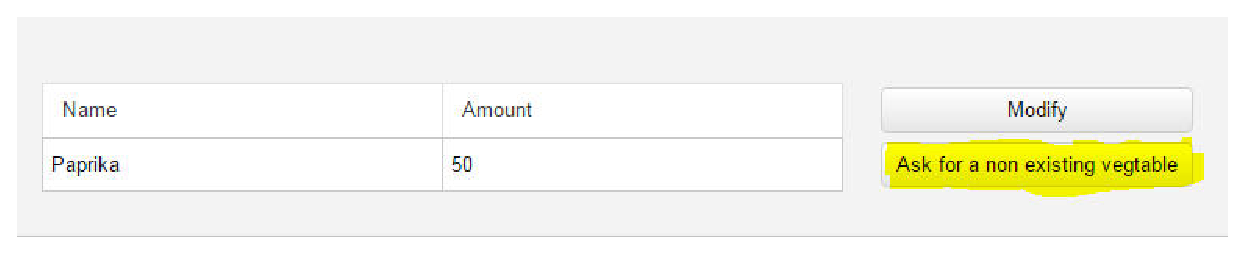
\includegraphics[width=1\textwidth]{images/AskForANonExistingVegtable.eps}
\end{figure}
\item \textbf{System} displays a pop up of the entered information.
\begin{figure}[H]
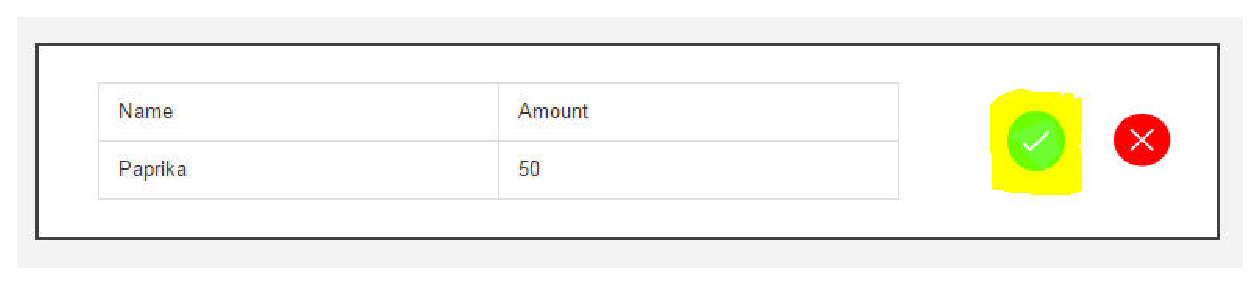
\includegraphics[width=1\textwidth]{images/AskForANonExistingVegtablePopUp.eps}
\end{figure}
\item \textbf{Gardener} accepts the pop up.
\item \textbf{System} pushes the information to the manager request seed table
and updates it.
\end{enumerate}
\end{description}

\subsubsection{Example of asking a diffrent seed}
\textbf{Technician} complets the given input text fields with the Name Mango and
amount 50. \textbf{System} displays the pop up of the information enterer Mango
and 50.\textbf{Gardener} accepts the pop up.\textbf{System} updates the request
crop table by adding Mango and amount to the table.
\hfill
\vspace{0.5cm}
\hrule

\break

\subsection{Modify/Retrive seed Amount}

\hrule
\hfill
\vspace{0.5cm}
\label{operation:modifySeedAmount}


The \textbf{Gardener} can modify the amount of seed on the crops inventory
table.
\begin{description}
\item \textbf{Parameters:} Name,amount
\item \textbf{Precondition:} The system is bootedup and the gardener has to be
logged in and be on the Gardener sreen.
\item \textbf{Post-condition:} Seed inventory has been modifyed on manager and
gardener screen.
\item \textbf{Output messages:} Successfully retrived seeds from inventory
\item \textbf{Triggering:}
\begin{enumerate}
\item \textbf{Gardener} Complets the input text fields and presses the modify
button.
\begin{figure}[H]
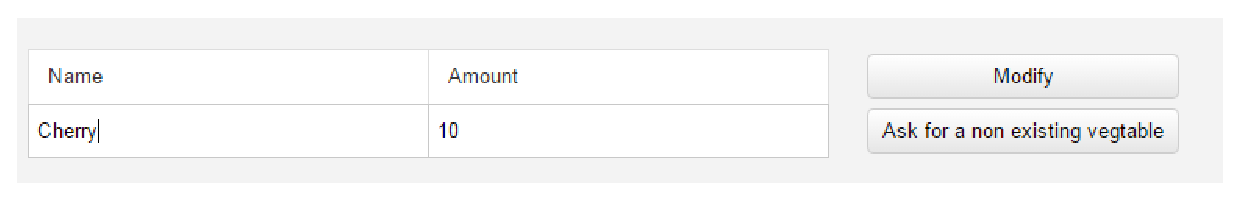
\includegraphics[width=1\textwidth]{images/RetriveCropsBase.eps}
\end{figure}
\item System updates the table of seed inventory and adds a the time of
retriving to the manager retriving Gardener table adn reloads the screen.
\end{enumerate}
\end{description}

\subsubsection{Example of removing crops}
\textbf{Gardener} enters the two input fields name = Tomatoe and amount=10.
The system retrives the amount which is equal to 10 from the inventory amount of
the name Tomatoe.
\hfill
\vspace{0.5cm}
\hrule


\subsection{Ask System for a suggestion}
\hrule
\hfill
\vspace{0.5cm}
\label{operation:AskSystemForASuggestion}

The \textbf{Gardener} can ask the system for a sugestion to place the seed in a
given room.
\begin{description} 

\item \textbf{Parameters:} SeedName
\item \textbf{Precondition:} The system is bootedup and Gardener has to be
logged in and be on the Gardener home screen.
\item \textbf{Post-condition:} A message is returned which displays in which
room the seed has to be placed.
\item \textbf{Output messages:} I suggest to Place it in room (1-4).
\item \textbf{Triggering:}
\begin{enumerate}
\item \textbf{Gardener} pressed the ask me button.
\item System displays a message for the given room where the seed needs to be
placed.
\end{enumerate}
\end{description}

\subsubsection{Example of Ask the system for a sugestion}
\textbf{Gardener} Enters in the input field Apple and presses the button ask me.
As a result the system will display a suggestionwhere the seed needs to be
placed.In this case the system suggest to place it in room 1.

 \hfill
\vspace{0.5cm}
\hrule



